\documentclass[a4paper]{article}
\usepackage[top=0pt,bottom=0pt,left=0pt,right=0pt]{geometry}
\usepackage{tikz}
\usepackage[math-style=ISO,bold-style=ISO,mathrm=sym]{unicode-math}

\defaultfontfeatures{Ligatures=TeX}
\setmainfont[BoldItalicFont=Linux Biolinum Slanted Bold]{Libertinus Sans}
\setmathfont[NFSSFamily=mathfont,RawFeature={+ss08}]{Libertinus Math}
\DeclareMathAlphabet{\mathcal}{OMS}{cmsy}{m}{n}

\Umathcode "31 = "0"0"1D7E3
\Umathcode "32 = "0"0"1D7E4
\Umathcode "33 = "0"0"1D7E5
\Umathcode "34 = "0"0"1D7E6
\Umathcode "35 = "0"0"1D7E7
\Umathcode "36 = "0"0"1D7E8
\Umathcode "37 = "0"0"1D7E9
\Umathcode "38 = "0"0"1D7EA
\Umathcode "39 = "0"0"1D7EB
\Umathcode "30 = "0"0"1D7E2

\pagestyle{empty}

\begin{document}

\noindent\begin{tikzpicture}

\clip (0,0) rectangle +(21,29.7);

\foreach \x in {11,38,...,199} \foreach \y in {15,42,...,260}
{
\begin{scope}[shift={(\x/10+1.25,\y/10+1.25)}]
%\draw (0,0) circle (12.5mm);
\node at (0,0) {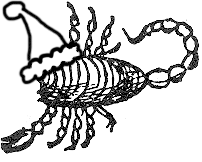
\includegraphics[width=10mm]{scorpion}};

\foreach \l/\a in {p/-49.5,a/-40.5,c/-32.5,k/-24,o/-11.5,f/-4,5/7.5,c/17.5,a/26,r/33.5,d/41.5,s/49.5}
{
\begin{scope}[rotate=\a] \node[rotate=\a] at (0,-10mm) {\vphantom{packof5cards}\l}; \end{scope}
}
\end{scope}
}

\end{tikzpicture}


\end{document}
